\documentclass{article}
\usepackage[utf8]{inputenc}

\title{Use of asynchronous circuits and leakiness in modeling biological circuit of the Caulobacter Crescentus cell cycle}
\author{Zoey Zhou}
\date{\today}  
\usepackage{graphicx}
\graphicspath{ {c:/Users/cuizy/Downloads/} }
\usepackage{amsmath}
\begin{document}

\maketitle

\section{Intro}
Biological modeling uses from stochastic to continuous to boolean models.  We propose an asynchronous circuit scheme for modeling the cell cycle of the bacteria Caulobacter Crescentus.   Asynchronous circuits are a type of digital circuits where the values are boolean, either 0 or 1, and the boolean functions are implemented through logic gates.  Digital circuits can be synchronous, where all of the logic gates in the circuit are controlled by some global clock, which ensures that the next values for all of the gates are updated at the same time.  Thus problems where various gate delays causing fluctuations in the circuit can be avoided.  In an asynchronous circuit, there is no global clock, and the gates update real time so different computational delay times for each gate cause real effects which may be propagated through the circuit.  Thus for an asynchronous circuit to provide reliable function, these random delays must be designed into the system.  A more stringent condition of asynchronous circuits known as speed independence ensures that no matter the delay for each gate, the circuit will function the same way. 
% different levels of detail

\section{Correct boolean model}
Current designs of digital circuits use mostly synchronous circuits.  They are called synchronous due to the existence of a global clock which controls each logic gate.  The clock signals ensures that each gate are updated at the right time, synchronously, and also are given enough time to process the inputs into the correct output to the next gate. This avoids transmitting the wrong intermediate signal, which can cause an error in the final output compared to what we would expect.  There are also asynchronous circuit designs, where there are no such clocks and each gate may finish processing its inputs at random.  The delay times, the time from when an input is applied until the proper output is reached, is thus variable.  This may cause certain transitions to happen before others at one time, and later than other during another processing of the inputs.  Depending on the circuit topology, changing the order of when these outputs are available may change the final logic output, usually an event that we would like to avoid if we want the circuit to perform reliably.  Thus asynchronous systems must be designed more carefully to allow for these random events.  To understand how digital circuits and especially asynchronous digital circuits are designed, we first look at the pieces from the ground up.  We review the basics of a complementary metal-oxide-semiconductor (CMOS) circuit, what digital circuits mean and some general properties for digital circuits to function.
\newline \newline
%expand more about continuous to binary (check)
The inputs and outputs of electronic devices are voltage values which are continuous for example can take any value between a minimum value like 0 V and some maximum value $V_{max}$ .  Circuits that operate using these continuous values to transmit signals and therefore information are called analog circuits.  Digital circuits are an abstraction on top of these underlying analog circuits.  They restrict the information passed by the signals so that the continuum of possible values for the signal are not all significant.  Only two values are allowed in digital circuits, '1' or '0'.  The binary value of'1' or '0' is extracted from the original analog signal by thresholds.  Usually there is a low and a high threshold, and an in between region.(figure)  If the signal is below the low threshold then it is a binary '0' and if the signal is above the high threshold it is a binary '1'.  The in between region is undetermined meaning it is neither a '1' or a '0'.  For this reason a digital value of high or '1' are synonymous and also represented in the circuit by a high voltage value.  The same is true of a digital value of low or '0' is represented in the circuit by a low voltage value.  There are many reasons why we would want the drastic reduction of the amount of information carried from an analog system to a digital system.  The main reasons are due to process variation when fabricating these devices and noise.  Variation means that each device does not function exactly as how it is specified, but each has some percentage difference between its true value and the design.  Noise degrades the signal, and makes it hard to use the raw analog signal, for example when adding two numbers together.  Digital circuits greatly reduce these issues because instead of the actual value, only a high or low signal matters.
\newline
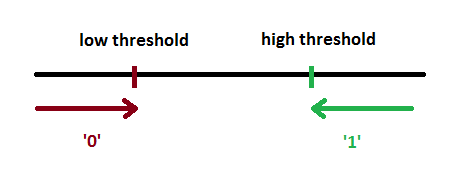
\includegraphics[width=\textwidth]{thresholds}
\newline
Present day circuits generally use metal–oxide–semiconductor field-effect transistors (MOSFETs) in their designs.  These devices has three connections, the gate, the drain and the source.  The gate allows some voltage to be applied over the device but is not actually connected to the drain or the source.  Depending on the relative voltage of the gate and source and drain and source, the drain and source may have no current flowing between them, effectively functioning as an open circuit, or approximately as a resistor.    
%do I need to go in more detail?
\newline
\begin{center}
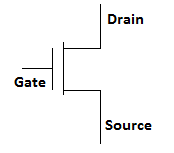
\includegraphics{mosfet}
\end{center}
\newline \newline
In CMOS there is the concept of a pull up network and a pull down network.  Based on the logic of the pull up and pull down networks, they can either function as an open in the circuit, or as some connective component.  So that when the pull up network is connected, and when the pull down network is effectively an open, the output signal gets pulled high.  While if the pull down network is connected and the pull up network is an open, the output signal gets pulled low.  In the inverter example, the pull up network consists of a PMOS that is connected to a voltage supply of $V_{dd}$ on one end and the pull down network consists of a NMOS which is connected to ground on one end.  PMOS behaves, on first order approximation, as a resistor when the input voltage is low and as an open switch when the input voltage is high.  NMOS is the opposite, it behaves as an open switch when the input voltage is low and as a resistor when the input voltage is high.  Thus when the input voltage is low, the output voltage is pulled up by the PMOS to $V_{dd}$.  Meanwhile when the input voltage is high, the output voltage is pulled down to ground by the NMOS.  The voltage transfer characteristic (VTC) of the inverter is a sigmoid.  This can be worked out using the equations of the MOSFET in different regions of operation.  It is in fact also a sigmoid in the other boolean logic gates that we use such as AND and OR gates.
%(write about dynamic memory later?)
\newline \newline
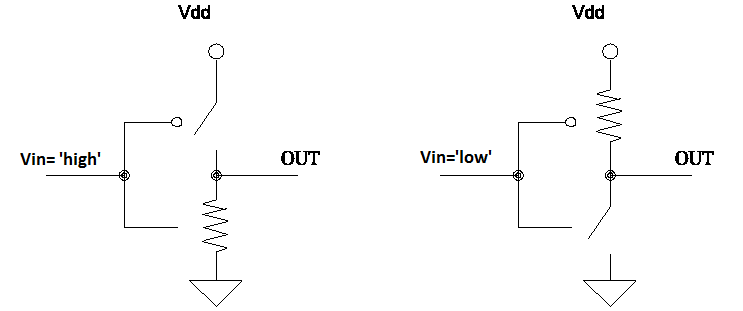
\includegraphics[width=\textwidth]{mosinaction2}
\begin{center}
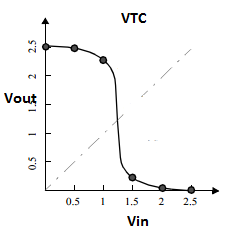
\includegraphics{vtc}
\end{center}
\newline \newline

Memory elements are important in asynchronous circuits because they can hold the signal for some time until they receive input, usually from elements further down the circuit to signal that the current output has been acknowledged and processed already and does not need to hold anymore.  This can be implemented in a number of ways but one method is adding a capacitor to the output.  The equation of a capacitor is 
\[I(t)=C\frac{dV(t)}{dt}
\]
It can be thought of as being charged up by the voltage as a high voltage is applied from $V_{out}$, or discharges when $V_{out}$ is low.  When in an RC circuit, the capacitor charges and discharges exponentially.  This is a valid way of maintaining the output voltage at either high or low for short amounts of time. 
\begin{center}
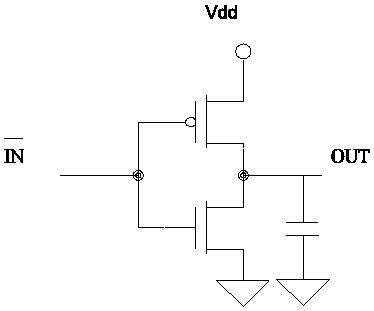
\includegraphics{mosinv}
\end{center}

\newline
%This is generic... can be applied to both
We must also verify some properties when these circuit components are connected to each other.  To ensure that they operate correctly as part of a larger circuit. First we want verify the thresholds are upheld so that for all signals below the low threshold, it is read into the gate as a '0' and produces the correct corresponding output.  This must be verified for all signals above the high threshold as well. We first work with a single input and make some assumptions:  1) that passing the signal at the low and high threshold though the gate produces the proper binary output signal, 2) the gate function is a monotonic function.  Then all inputs below the input low threshold or above the input high threshold gives valid output signals as well.  We first assume the function G() is monotonically increasing, the reasoning is that for all $input low$ $x_i$ pairs, where $input low>x_i$ then $G(input low)>G(x_i)$.  The same could be shown for $input high$ and $x_j$.  If the function G() is monotonically decreasing then the inequality sign of the previous argument is flipped and the correct operation of the circuit still holds.  (We verify that our initial assumptions hold in that we can set the output low and high thresholds accordingly, and sigmoidal functions are indeed monotonic functions. )
%there are actually examples where this fails 0->0 in monotonically decreasing... need to fix too
\newline \newline
The next step is when gates are connected to each other, signals must propagate meaningfully as well.  The output of a gate should read as the same binary value into the input of the following gate based on their respective thresholds.  That is for the $i^{th}$ component which is connected to the $i+1^{th}$ component, $output_i low \leq input_{i+1} low$ and $output_i high \geq input_{i+1} high$.  Multiple inputs are common in biology where there can be activators and repressors and even degradation enzymes involved in one gene product.  This is easily reducible to the familiar problem in one dimension. 
\newline \newline
The other property that sigmoidal curves are important for is the restorative property of signals to allow for noise and increase robustness.  For the signals to allow a certain amount of noise to enter the system, we would want the output thresholds of one gate to be as far away from the input thresholds of the next gate as possible.  Thus when noise gets added to the output signal, it still has a good chance to transmit the correct binary data to the next stage.  In addition, these components can be connected in a loop.  In electronics, since the outputs and inputs are measured against the same unit of measurement, the voltage, the additional requirement is that the gain must be greater than 1.  This means that the slope of the function should be greater than 1.  
\newline \newline 

\section{Dynamic Memory}
%some intro about memory?
%EE
We have seen in the previous section how short term memory elements can be implemented with capacitors.  We examine some other ideal memory elements we would like as part of an asynchronous circuit, such as the Muller C-element. 
The Muller C-element is useful in the design of asynchronous circuits.  If every signal in a circuit is connected with C-elements then it ensures that the circuit can run robustly and has the speed independence property.  Thus we would ideally want the elements we see in biological circuits to operate similarly to the C-element.  A common CMOS implementation of a C-element is shown with two inputs A and B, and an output C.  It operates similarly as the inverter example.  In this C-element example, when A and B are both high, the pull down network is activated, while there are open switches in the pull up network and the output is connected to the ground.  When both A and B are low, the opposite is true and the output is pulled to $V_{cc}$.  However when A and B are different signals ie A is high and B is low or when A is low and B is high, then there is no path through either the pull up or the pull down network and the previous value of the output is retained.  This state is called a 'hold'.
\begin{center}
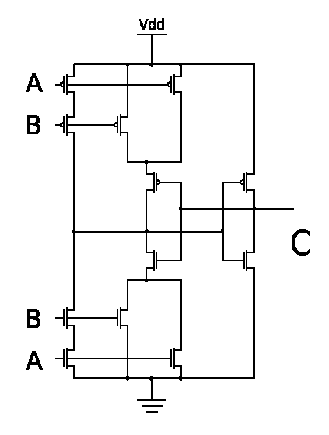
\includegraphics{celement}
\end{center}
\begin{center}

\begin{tabular}{|p{1.5cm}|p{1.5cm}|p{1.5cm}|p{2cm}| } 
 \hline
\textbf{In1} & \textbf{In2} & \textbf{Qnext} & \textbf{Action} \\
\hline
1 & 1 & 1 & set \\
\hline
0 & 0 & 0 & reset \\ 
\hline
0 & 1 & Q & hold state \\ 
\hline
1 & 0 & Q & hold state\\ 
\hline
\end{tabular}

\end{center}

\newline
%EE
Set reset latches have a similar modes of operation with output high output low and hold but also differs in an important detail.  In a set reset latch, there are two inputs, called a set and a reset.  We look at the set reset NOR latch.  When set is high and reset is low then the output signal is 'set' or becomes high.  When set is low and reset is high then the output signal is 'reset' or becomes low.  If both inputs are low then the output does not change and is in the hold state.  The last state when both inputs are high gives an undefined output represented by 'X', usually this element does not go into this state.  The similarities between set reset latches and C-elements are quite apparent.  It is basically equivalent if you treat the reset signal of the set reset latch as an inverted second signal for the C-element.  However, when A is high and B is low, there is a hold state for the C-element whereas that corresponds to a high set and high reset and thus an undefined output for the set reset latch.
\begin{center}

\begin{tabular}{|p{1.5cm}|p{1.5cm}|p{1.5cm}|p{2cm}| } 
 \hline
\textbf{S} & \textbf{R} & \textbf{Qnext} & \textbf{Action} \\
\hline
1 & 0 & 1 & set \\
\hline
0 & 1 & 0 & reset \\ 
\hline
0 & 0 & Q & hold state \\ 
\hline
1 & 1 & X & not allowed\\ 
\hline
\end{tabular}

\end{center}


\section{Biology equivalent}
%BIO
We expect biological systems to behave similarly to an asynchronous circuit because in biological systems there are no 'global clocks' that regulate the timing.  Because there is high variability between cells, and molecular interactions are of a stochastic nature, production from each gene element can have varying delay.  This variability differs from cell to cell and from one cycle to the next. Thus we would also expect a type of speed independence property to ensure that most of the time, the cells work reliably regardless of the random delays and advance through the cell cycle to produce new cells.
\newline \newline
%BIO
From the bottom up, we extract properties from biological networks and use analogies with the well developed CMOS technology.  We start at the molecular level and demonstrate certain properties so that we can group gene elements together and represent them with a higher level boolean model.  We then show how this boolean model can be abstracted into a higher level forming building blocks that we can use in an asynchronous circuit. 
\newline \newline
%BIO
The physics of gene protein interactions in the cell are congruent with properties that make it a valid digital circuit as well.  In past papers, gene regulatory networks has been modeled as boolean circuits with each gene/protein element represented by a boolean logic gate.  Each gene logic gate has inputs, such as activators and repressors, to determine whether the protein is being actively produced or not.  The mRNA production here can be modeled with the Hill function.  The sigmoidal shape of the Hill function is reminiscent of VTC of CMOS gates.  As such, much of the design properties of CMOS circuits can be carried over.  There are two important properties that gates, which we use as building blocks in circuits, must satisfy.  The existence of a threshold, and the faithful propagation of a signal through a circuit, even when connected in a loop.  We examine these properties by first looking at the steady state solution of the equation for protein production.  The steady state solution is important because within a reasonable amount of time this is the output concentration of the protein given the inputs. This sigmoidal curve is then an input (the proteins that initiate transcription and production of the protein) versus the output, the current concentration of the protein.  The sigmoidal shape of the input vs output transfer curve during steady state allows for restoring property of the signal and hence faithful propagation in its next stages.   In an ODE model of the protein production and degradation with the Hill function, the steady state solutions are the Hill function divided by the degradation constant.  In general the protein production equation is of the form: $\frac{dprotein}{dt}=g(inputs)-protein\cdot\lambda$  where the function $g()$ is a sigmoidal curve such as the Hill function and $\lambda$ is the degradation constant.  It's steady state solution is $protein=g(inputs)/\lambda$, easily verifiable as also a sigmoidal Hill function.
\newline \newline
%BIO
 In biological systems where the ODE model is a sigmoidal curve in the form of a Hill function, the partial derivative with respect to any one input variable is always monotonic.  Thus this satisfies our monotonic requirement from the analysis in the previous section and ensures that proper propagation occurs through the circuit with the appropriate choices of thresholds. % In addition, because these equations are monotonic with regard to any one variable, there are only a limited number of logic that can be formed.  (expand?)
%BIO
%\newline \newline
%Because we are using different chemical species at each stage to transmit the biological signal, we need to scale the slopes of the function accordingly.  
%Sigmoidal, All the things about how they connect, why they are good latches/ memory elements, completion signals?
\newline \newline
%BIO
Changing rates of degradation of proteins is an important aspect of the circuit that has been often ignored in previous models.  In past papers, gene regulatory networks has been modeled as boolean circuits with each gene/protein element represented by a boolean logic gate.  Each gene logic gate has inputs, usually its activators and repressors, to determine whether the protein is being actively produced or not.  These are usually modeled as AND or OR gates with its promoter binding compounds as its only inputs.  However, in our investigation using the ODE model of each gene, we found that degradation is a crucial part of the logic gates as well.  Protein degradation can be sped up through controlling the production of degradation enzymes.  Meanwhile for stable proteins, it is possible for the base degradation rate, the half life of the protein to be equivalent to the length of the cell cycle, the only reduction in protein concentration coming from the splitting of cells.  These proteins, once produced would remain in the cells for a very long time and essentially considered 'on' even when transcription and/or translation has stopped.  Thus there needs to be a separate way of representing the production of proteins from its degradation.  We take inspiration from CMOS technology.  We recall that CMOS employs pull up networks and pull down networks to produce an output value of either high or low.  The transcriptional and translational regulation of genes are similar to a pull up network while the accelerated degradation is similar to a pull down network.  If the background degradation is significantly slower, this effect can be thought of as similar to the parasitic capacitance that slowly leak the charge of the output signal.  Overtime it degrades the output signal however for short time scales the output retains its voltage value and can be considered a dynamic memory element. 

There are certain network motifs in biology that allows cells to have some sort of memory.  Our main examples are from Caulobacter but these motifs are present in other cells and thus this analysis is widely applicable.  
%There are positive feedback loops such as in CtrA where once enough production of CtrA starts the feedback, it will remain locked in that high state.  Until degradation overpowers the feedback and pulls CtrA back down to a low state.  This bistable property is also how latches in digital circuits store memory. 
We take inspiration from dynamic memory and look into the short term behavior of each gate.  As mentioned in the previous section, when the degradation term is slow, the changes in protein concentration over time is slow as well.  For very stable proteins, the half life of the protein is then only from splitting of the cells during each cell cycle.  We examine whether using experimentally determined parameters, it is possible to view these gates as memory elements.  For our analysis, we assume that the inputs are held constant.  Then there is a closed form exponential solution of our ODE model.  We can then determine the time elapsed from a given starting state to a final state.  (z is the output protein concentration, and c is the total contribution by the inputs, a constant if the inputs are held constant, $\lambda$ is the degradation rate)
\[\frac{dz}{dt}=c-z\cdot\lambda
\]
The solution to this ODE is the exponential:
\[z(t)=((z_0\cdot\lambda-c)e^{(-\lambda\cdot t)}+c)/\lambda
\]
Where $z_0$ is the inital concentration of the protein.  To find the time elapsed between $z_0$ and some $z_f$ just substitute $z(t)=z_f$.  We also note that at steady state $c=z_{ss}\cdot\lambda$.  Rearranging the equation for time:
\[\Delta t= -log(z_f-z_{ss})/ \lambda+ log(z_0-z_{ss})/ \lambda
\]
or
\[\Delta t= -log(z_{ss}-z_f)/ \lambda+ log(z_{ss}-z_0)/ \lambda
\]
because the expression inside the log must be positive.  (Note that this means $z_f$ and $z_0$ must be on the 'same side' as $z_{ss}$, this makes conceptual sense because this is an exponential decay or rise towards the final steady state value, it cannot cross the steady state value.)
 This is the amount of time it takes where $z_0$ is the initial protein concentration and $z_f$ is the final protein concentration.
\newline
%something about robustness?

\newline  \newline
In our model we wish to verify the set reset and hold property of each gene gate.  We use the exponential solution to the ODE equation.  Given the appropriate inputs we would like for all of the set and and reset transitions to take a shorter length of time than the temporary hold states.  More formally, we would like the worst case/longest set and reset transition times to be shorter than the worst case/shortest hold times.  First we define some of the parameters and variables that we use.  Define the input thresholds as:  $in_{min0}$ is the smallest acceptable input to represent an input '0' and $in_{max0}$ is the largest acceptable input to represent an input '1'.  Similarly, $in_{min1}$ is the smallest acceptable input to represent an input '1' and $in_{max1}$ is the largest acceptable input to represent an input '1'.  $fanout_0$ and $fanout_1$ represent the '0' and '1' input thresholds to the next components respectively.  There is an additional constraint where fanout thresholds $fanout_0$ and $fanout_1$ must be between $g(in_{max0})$ and $g(in_{min1})$ so that all legal input values provide legal outputs that feed into the next layer of components to be processed.
\newline \newline
To find the maximum and minimum times for set reset and hold, we analyze the equation for time.  To find the maximum set time, since set is when the output rises from '0' to '1' we can assume that $z_{ss}>z_f, z_0$ and use the second form of the time equation. $\Delta t$ is monotonically increasing in $z_f$ and monotonically decreasing in $z_0$.  Since $z_{ss}$ is involved in two terms we need further analysis to see its effects on time.  Taking the derivative with respect to $z_{ss}$:
\[\frac{d\Delta t}{dz_{ss}}=- \frac{1}{(z_{ss}-z_f)}\frac{1}{\lambda}+ \frac{1}{(z_{ss}-z_0)}\frac{1}{\lambda}
\]
To find the maximum set time, we want to use the maximum $z_f$ where $z_f$ crosses the threshold to become a '1' signal and the minimum $z_0$ where $z_0$ is a '0' signal.  So we have $z_f=fanout_1$ and $z_0=g(in_{min0})$ using the monotonicity of the function g().  $z_{ss}$ is the steady state achieved by some constant input.  This input must be a valid '1' input so that set occurs and the steady state is also a valid '1' output.  Thus $z_{ss}$ must be bounded by: $g(in_{min1})\leq z_{ss}\leq g(in_{max1})$, and from earlier constraints we know that $fanout_1<z_{ss}$ and $fanout_1>g(in_{min0})$ so that:
\[z_{ss}-fanout1< z_{ss}-g(in_{min0})
\]
\[\frac{1}{z_{ss}-fanout1}>\frac{1}{z_{ss}-g(in_{min0})}
\]
The derivative $\frac{d\Delta t}{dz_{ss}}$ is always negative in this case, so the smallest possible value in $z_{ss}$'s domain maximizes the set time, which is $z_{ss}=g(in_{min1})$.
%insert some graph here
The maximum time for a set to occur can be rewritten as:
\[\Delta t_{set}= - \frac{1}{\lambda} log(g(in_{min1})-fanout_1)/(g(in_{min1}) -g(in_{min0}))
\]
Next we find the maximum reset time.  (output goes from '1' to '0' while an input '0' is applied)  Since it is an exponential decay, we use the first formula for time.  $\Delta t$ is monotonically decreasing in $z_f$ and monotonically increasing in $z_0$.  Again take the derivative of the time equation with respect to $z_{ss}$:
\[\frac{d\Delta t}{dz_{ss}}= \frac{1}{(z_f-z_{ss})}\frac{1}{\lambda}- \frac{1}{(z_0-z_{ss})}\frac{1}{\lambda}
\]
To find the maximum reset time, we want to use the minimum $z_f$ where $z_f$ crosses the threshold to become a '0' signal and the maximum $z_0$ where $z_0$ is a '1' signal.  So we have $z_f=fanout_0$ and $z_0=g(in_{max1})$ using the monotonicity of the function g().  $z_{ss}$ is an output '0' valued steady state achieved by a constant input that is also a valid '0' on the input side.  Thus $z_{ss}$ must be bounded by: $g(in_{min0})\leq z_{ss}\leq g(in_{max0})$, and from earlier constraints we know that $z_{ss}<fanout_0$ and $fanout_0<g(in_{max1})$ so that:
\[fanout0-z_{ss}< g(in_{max1})-z_{ss}
\]
\[\frac{1}{fanout0-z_{ss}}>\frac{1}{g(in_{max1})-z_{ss}}
\]
The derivative $\frac{d\Delta t}{dz_{ss}}$ is always positive in this case, so the largest possible value in $z_{ss}$'s domain maximizes the set time, which is $z_{ss}=g(in_{max0})$.
The maximum time for a set to occur can be rewritten as:
\[\Delta t_{reset}= -\frac{1}{\lambda} log(fanout_0 –g(in_{max0}))/(g(in_{max1}) – g(in_{max0}))
\]
For holds we want a minimum bound on the time the output remains within the '0' or '1' regions as the inputs are changed.  We first look at how long a signal stays in the '0' region, or the hold 0 case.  We assume that the output eventually rises from the initial '0' value so that $z_{ss}>z_0$.  Note that if $z_{ss}<fanout_0$ then the output signal will be held at '0' indefinitely.  So we look at the case where $z_{ss}>fanout_0$.  Similar to finding the set time, we use the second form of the time equation.  This time we would like to find the minimum value for the time.  Since $\Delta t$ is monotonically increasing in $z_f$ and monotonically decreasing in $z_0$, we want to use the minimum $z_f$ such that the output stops being a valid '0' signal, that is $fanout_0$, and use the maximum $z_0$ that is a valid input '0', that is $g(in_{max0})$.  Additionally since the derivative of this equation with respect to $z_{ss}$ is always negative, we apply the largest possible 'hold' input where both active production and degradation are still considered '0'.  That is the baseline degradation and $in_{max0}$.  Because the degradation is different, the value $z_{ss}$ differs from $g(in_{max0})$, the input output pair has a different transfer function, call it $g'()$ so that the steady state output is $g'(in_{max0})$
\[\Delta t_{hold0}= -\frac{1}{\lambda} log(g'(in_{max0}) -fanout_0)/(g'(in_{max0}) -g(in_{max0}))				
\]
The analysis is similar for the minimum time a signal stays in the '1' region, or the hold 1 case.  For this case the output eventually decays from the initial '1' value so $z_{ss}<z_0$. Again, if $z_{ss}>fanout_1$ then the output signal will be held at '1' indefinitely. So we look at the case where $z_{ss}<fanout_1$.  Similar to finding the reset time, we use the first form of the time equation.   We would like to find the minimum value for the time.  Since $\Delta t$ is monotonically decreasing in $z_f$ and monotonically increasing in $z_0$, we want to use the maximum $z_f$ such that the output stops being a valid '1' signal, that is $fanout_1$, and use the minimum $z_0$ that is a valid input '1', that is $g(in_{min1})$.  Additionally since the derivative of this equation with respect to $z_{ss}$ is always positive, we apply the smallest possible 'hold' input where both active production and degradation are still considered '0'.  That is the baseline degradation and $in_{min0}$.  Again due to the difference in degradation rate, we use a different input output transfer function $g'()$ so that the steady state output is $g'(in_{min0})$  
\[\Delta t_{hold1}= -\frac{1}{\lambda} log(fanout_1 -g'(in_{min0}))/(g(in_{min1}) -g'(in_{min0}))
\]
We check the function of the gcrA gene module against these equations.  We use parameter values that were previously determined for the ODE model from both experimental data and reasonable approximations based on these experiments.  
\begin{center}

\begin{tabular}{|p{1.8cm}|p{1cm}|p{1cm}|p{7cm}| } 
 \hline
\textbf{Parameter} & \textbf{Value} & \textbf{Units} & \textbf{Parameter explanation} \\
\hline
$\lambda_{sw}$ & 10.5 & min & GcrA half-life in swarmer \\ 
\hline
$\lambda_{st}$ & 42 & min & GcrA half-life in stalked \\ 
\hline
$issw$ & 0 or 1 & & boolean value where 1 indicates cell is in the swarmer state \\
\hline
$p_{gcrA}$ & 2.2 & nM/s & Maximum synthesis rate of GcrA from the promoter \\ 
\hline
$c_{HalfCtrA}$ & 1760 & nM & Concentration of CtrA~P that yields half of the maximum expression of CtrA-regulated genes\\
\hline
$c_{HalfDef}$ & 660 & nM & Default concentration of transciption factors ie. gcrA that yields half of the maximum expression of target genes\\
\hline
\end{tabular}

\end{center}
The equation for the ODE of just the gcrA gene module is:
\[
\begin{split}
\frac{d gcrA}{d t}=\frac{2.2}{(1+(\frac{660}{dnaA})^2)\cdot (1+(\frac{ctrAP}{1760})^2)}-gcrA\cdot (\frac{log(2)}{60\cdot 42} \\
+(issw)\cdot \frac{log(2)}{60\cdot 10.5})
\end{split}
\]
And the equation for the steady state is:
\[gcrA_{ss}=\frac{2.2}{(1+(\frac{660}{dnaA})^2)\cdot (1+(\frac{ctrAP}{1760})^2)\cdot (\frac{log(2)}{60\cdot 42}
+(issw)\cdot \frac{log(2)}{60\cdot 10.5})}
\]
The various input and output thresholds that we use are:
\[in_{min0}: dnaA=0, ctrAP=1760  \Rightarrow g(in_{min0})=0, g'(in_{min0})=0
\]
\[in_{max0}: dnaA=150, ctrAP=0  \Rightarrow g(in_{max0})=267, g'(in_{max0})=393
\]
\[in_{min1}: dnaA=660, ctrAP=1760  \Rightarrow g(in_{min1})=2666 %wouldn't this be a pareto frontier thing?  NO because of the monoticities in each var
\]
\[in_{max1}: dnaA=1000, ctrAP=0  \Rightarrow g(in_{max1})=3800
\]
\[fanout_0=600
\]
\[fanout_1=1100
\]
With these set of parameters and thresholds the set rest and hold times are:
\[\Delta t_{set}=1934.23749
\]
\[\Delta t_{reset}=1716.50821
\]
\[\Delta t_{hold0}= inf
\]
\[\Delta t_{hold1}=3218.61297
\]
The minimum hold times here are longer than the maximum set reset times and so for short periods of time, this element can be considered as a set-reset memory element.  Since these are the worst possible bounds, in practice set reset times would be shorter and the hold times would be even longer.  Thus we can abstract these biological motifs as a series of dynamic memories connected to each other.

\section{Asynchronous circuits}
One important aspect of asynchronous circuit design is having memory elements.  This is because for a asynchronous circuit to be able to function, it must receive feedback signals from the next stage so that it knows if it needs to hold its current value, or if the next stage has received it's signal and can go to the next stage in processing.

\section{Leakiness}
Interestingly, there are a couple examples even in the Caulobacter cell where if you knockout one of the key components of the core cell cycle proteins that the rest of the cycle still tries to proceed.  For example, experiments where GcrA or CcrM has been deleted should halt the cell cycle since they start the transcription of CtrA and DnaA respectively.  However, it has been shown that after some delay DnaA and CtrA levels accumulate enough such that the cell can enter the next phase of the cycle.  This may be attributed to a base rate of leakiness from their promoters and other stochastic effects.  We analyze the likely causes of this observation.

CtrA has positive self-feedback.  Plotting the solutions of the Hill kinetics and a diagonal line, representing that all CtrA are phosphorylated to CtrAP during this feedback, shows that this causes CtrA to be bistable. (figure \ref{fig:ctrapc})  However if you include leakiness of the promoter, that shifts the curve of CtrAP vs CtrA up such that even in the presence of no CtrAP, there is still some CtrA produced from the base rate.  If the leakiness from the promoter is large enough, it can shift the curve up so much that there is only one stable point of the system, where ctrA is high. (figure \ref{fig:ctrapl}) This would explain why deletion of GcrA and the P1 promoter where GcrA binds to delays the accumulation of CtrA.  In an earlier paper \cite{compgenre} Michaelis-Menton (MM) kinetics was used.  In their model, they also observed a restart of CtrA even when the upstream transcription factor GcrA was not present.  This is because the MM curve produces only one stable equilibrium so CtrA will always go high if given enough time.

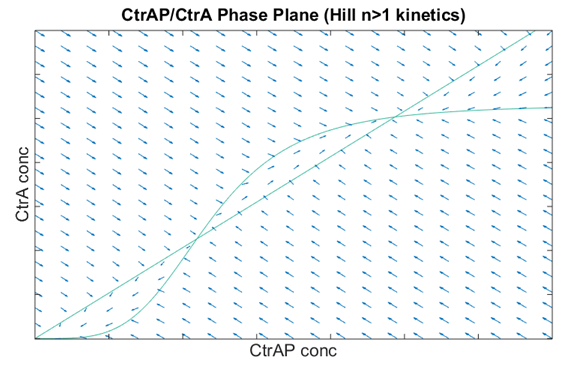
\includegraphics[width=\textwidth]{ctrapc}
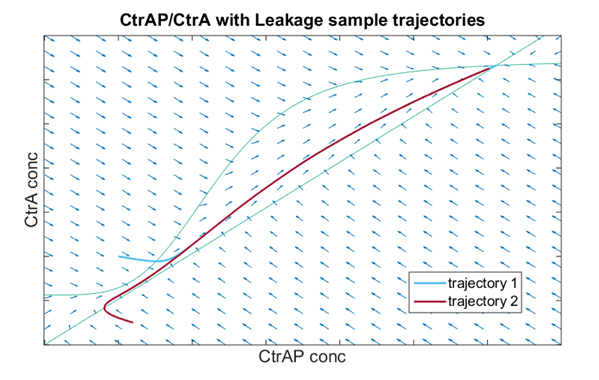
\includegraphics[width=\textwidth]{ctrapl}
\newline \newline
For DnaA, there is evidence that in cells with DnaA lacking the CcrM binding site, the phenotype is not as severe as deleting DnaA directly.  Instead the cell cycle is slowed down.  Thus, there is reason to believe that DnA is also controled by a leaky promoter.  

\begin{thebibliography}{9}
\bibitem{compgenre} 
S M Murray, G Panis, C Fumeaux, P H Viollier , M Howard. 
\textit{Computational and Genetic Reduction of a Cell Cycle to Its Simplest, Primordial Components}. 
PLOS Biology, December 31, 2013.
 
\end{thebibliography}
	
\end{document}
